% !TEX root = ../presentation.tex
% !BIB program = biber
% !TEX program = xelatex

\section[Extra Slides]{extra slides}


\subsection[Introduction]{introduction}


\begin{frame}
    \frametitle{Reliability of machine learning systems}
    \begin{itemize}
        \item <1-> \highlight{Data}: Quality, quantity, diversity, bias, privacy, ethics.
        \item <1-> \highlight{Task}: Context, domain, language, culture, purpose.
        \vspace{1em}
        \item <2-> \highlight{Interpretability} of how a model works (transparency, accountability, regulation).
        \item <2-> \highlight{Explainability} of model predictions (trust, understanding, feedback).
        \item <2-> \highlight{Fairness} in treatment of different groups of people.
        \item <2-> \highlight{Robustness} to noise, outliers, distribution shift, and adversarial attacks.
    \end{itemize}

    \note[item]{So what are the challenges holding us back in implementing such systems?}
    \note[item]{
        \begin{itemize}
            \item Strong requirements of data.
            \item Tasks that span different contexts, domains, languages, and cultures.
            \item Regulatory requirements for transparency and accountability.
            \item Trust and understanding of predictions.
        \end{itemize}
    }
\end{frame}


% ======================================================================================================================


\subsection[Hierarchical VAEs Know What They Don't Know]{hierarchical vaes know what they don't know}


\begin{frame}
    \frametitle{Hierarchy of speech features}
    \begin{figure}
        \centering
        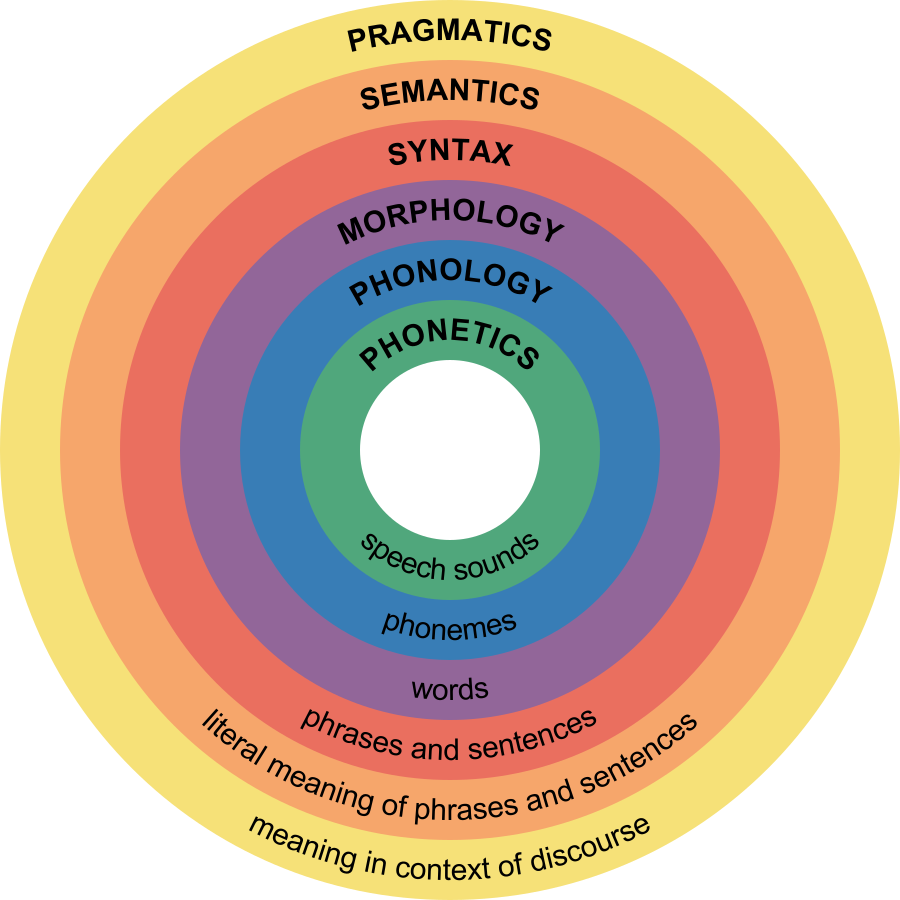
\includegraphics[height=\textheight]{figures/Major_levels_of_linguistic_structure.png}
    \end{figure}
\end{frame}


\begin{frame}
    \frametitle{Results on diverse datasets}
    \begin{columns}
        \begin{column}{0.45\textwidth}
            \hfill
            \begin{table}[t]
                \centering
                \resizebox{0.9\textwidth}{!}{%
                \begin{tabular}{llrrr}
                    \toprule
                    OOD dataset & Metric & AUROC$\uparrow$ & AUPRC$\uparrow$ & FPR80$\downarrow$ \\
                    \midrule
                    \multicolumn{5}{c}{\textbf{Trained on CIFAR10}} \\
                    \midrule
                    SVHN          &  $LLR^{>2}$  &  0.811  &  0.837  &  0.394  \\
                    CIFAR10       &  $LLR^{>1}$  &  0.469  &  0.479  &  0.835  \\
                    \midrule
                    \multicolumn{5}{c}{\textbf{Trained on SVHN}} \\
                    \midrule
                    CIFAR10            &  $LLR^{>1}$       &  $0.939$  &  $0.950$  &  $0.052$  \\
                    SVHN               &  $LLR^{>1}$       &  $0.489$  &  $0.484$  &  $0.799$  \\
                    \bottomrule
                \end{tabular}
                }
            \end{table}
            \hfill
        \end{column}
        \begin{column}{0.55\textwidth}
            \hfill
            \begin{table}[t]
                \centering
                \resizebox{0.9\textwidth}{!}{%
                \begin{tabular}{llrrr}
                    \toprule
                    OOD dataset & Metric & AUROC$\uparrow$ & AUPRC$\uparrow$ & FPR80$\downarrow$ \\
                    \midrule
                    \multicolumn{5}{c}{\textbf{Trained on FashionMNIST}} \\
                    \midrule
                    MNIST                    & $LLR^{>1}$             &  0.986  &  0.987  &  0.011 \\
                    notMNIST                 &  $LLR^{>1}$            &  0.998  &  0.998  &  0.000 \\
                    KMNIST                   &  $LLR^{>1}$            &  0.974  &  0.977  &  0.017 \\
                    Omniglot28x28            &  $LLR^{>2}$            &  1.000  &  1.000  &  0.000 \\
                    Omniglot28x28Inverted    &  $LLR^{>1}$            &  0.954  &  0.954  &  0.050 \\
                    SmallNORB28x28           &  $LLR^{>2}$            &  0.999  &  0.999  &  0.002 \\
                    SmallNORB28x28Inverted   &  $LLR^{>2}$            &  0.941  &  0.946  &  0.069 \\
    {\color{black!60}FashionMNIST}             &  $LLR^{>1}$            &  0.488  &  0.496  &  0.811 \\
                    \midrule
                    \multicolumn{5}{c}{\textbf{Trained on MNIST}} \\
                    \midrule
                    FashionMNIST                   &  $LLR^{>1}$  &  $0.999$  &  $0.999$  &  $0.000$ \\
                    notMNIST                       &  $LLR^{>1}$  &  $1.000$  &  $0.999$  &  $0.000$ \\
                    KMNIST                         &  $LLR^{>1}$  &  $0.999$  &  $0.999$  &  $0.000$ \\
                    Omniglot28x28                  &  $LLR^{>1}$  &  $1.000$  &  $1.000$  &  $0.000$ \\
                    Omniglot28x28Inverted          &  $LLR^{>1}$  &  $0.944$  &  $0.953$  &  $0.057$ \\
                    SmallNORB28x28                 &  $LLR^{>1}$  &  $1.000$  &  $1.000$  &  $0.000$ \\
                    SmallNORB28x28Inverted         &  $LLR^{>1}$  &  $0.985$  &  $0.987$  &  $0.000$ \\
    {\color{black!60}MNIST}                          &  $LLR^{>2}$  &  $0.515$  &  $0.507$  &  $0.792$ \\
                    \bottomrule
                \end{tabular}
                }
            \end{table}
            \hfill
        \end{column}
    \end{columns}
\end{frame}


% ======================================================================================================================


\subsection[A Brief Overview of Unsupervised Speech Representation Learning]{a brief overview of unsupervised speech representation learning}


\begin{frame}
    \frametitle{Types of self-supervised speech representation learning methods}
    
    Schematic of self-supervised methods. Each subfigure illustrates the loss computation for a single time-step. The temporal subscript has been left out for simplicity.

    \begin{figure}
        \centering
        \setlength\tabcolsep{1.5pt}
        \resizebox*{\textheight}{!}{%
        \begin{tabular}{>{\centering\arraybackslash} m{4mm}  >{\centering\arraybackslash} m{0.40\textwidth}|>{\centering\arraybackslash} m{0.40\textwidth}}
            & {\small \textsc{predictive}} & {\small \textsc{masking-based}} \\
            \rotatebox{90}{{\small \textsc{reconstruct}}} & 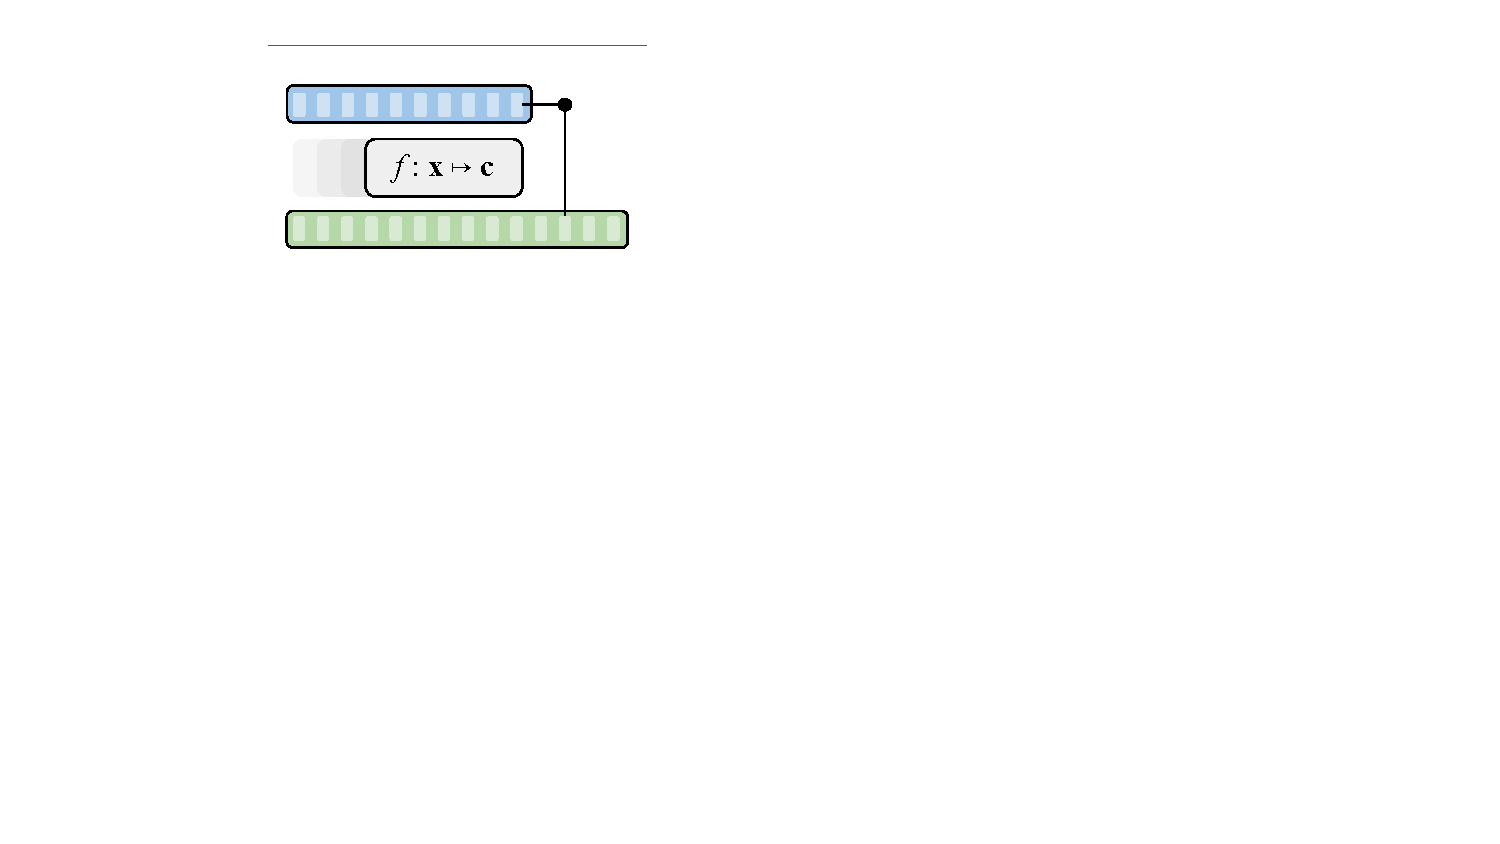
\includegraphics[width=0.40\textwidth]{../graphics/paper_brief/REC_PRD.pdf} & 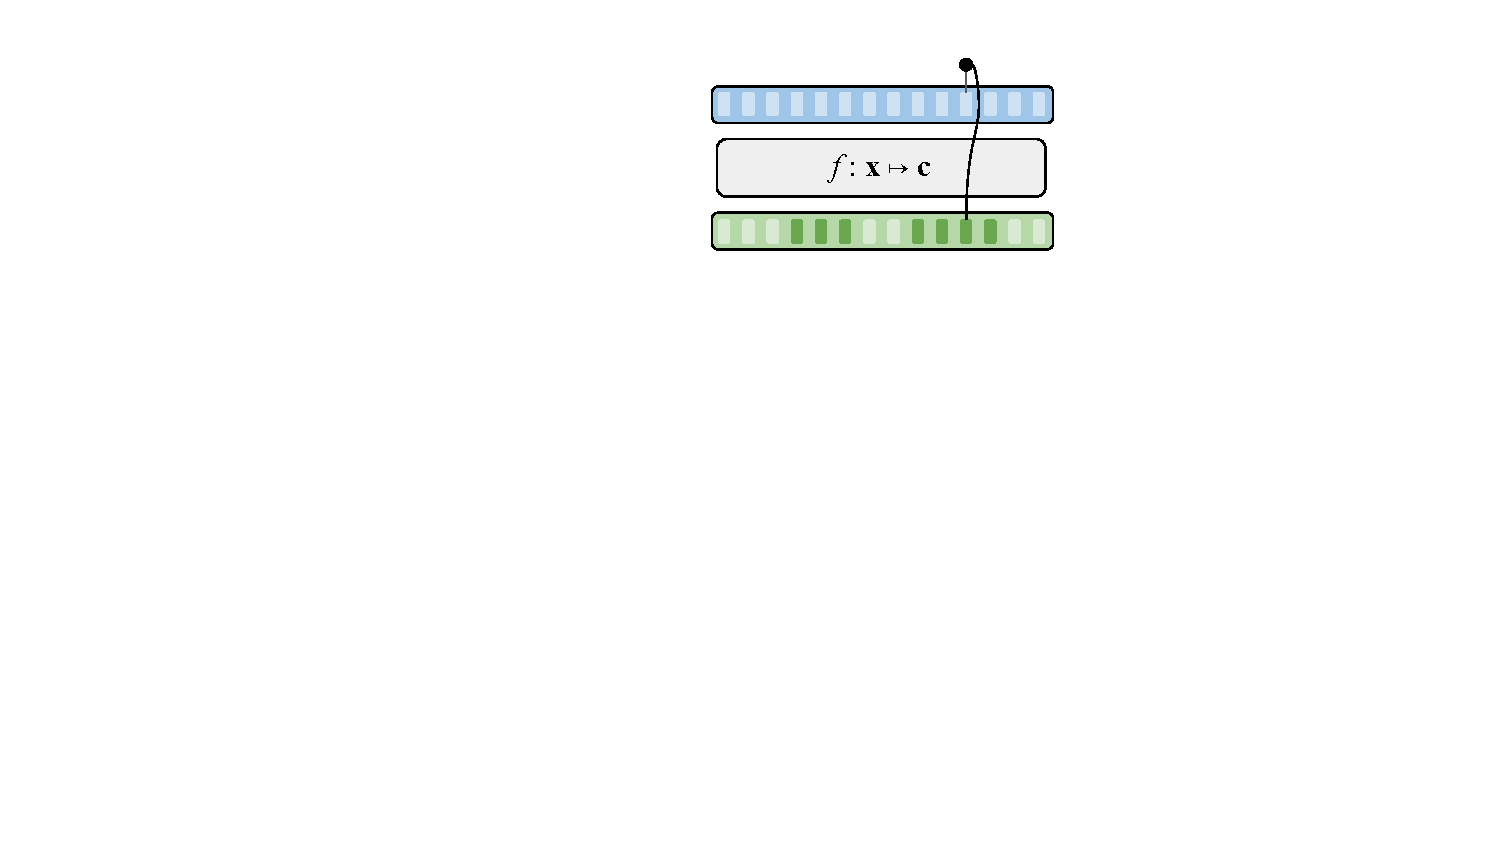
\includegraphics[width=0.40\textwidth]{../graphics/paper_brief/REC_MSK.pdf}  \\
            \midrule
            \rotatebox{90}{{\small \textsc{contrastive}}} & 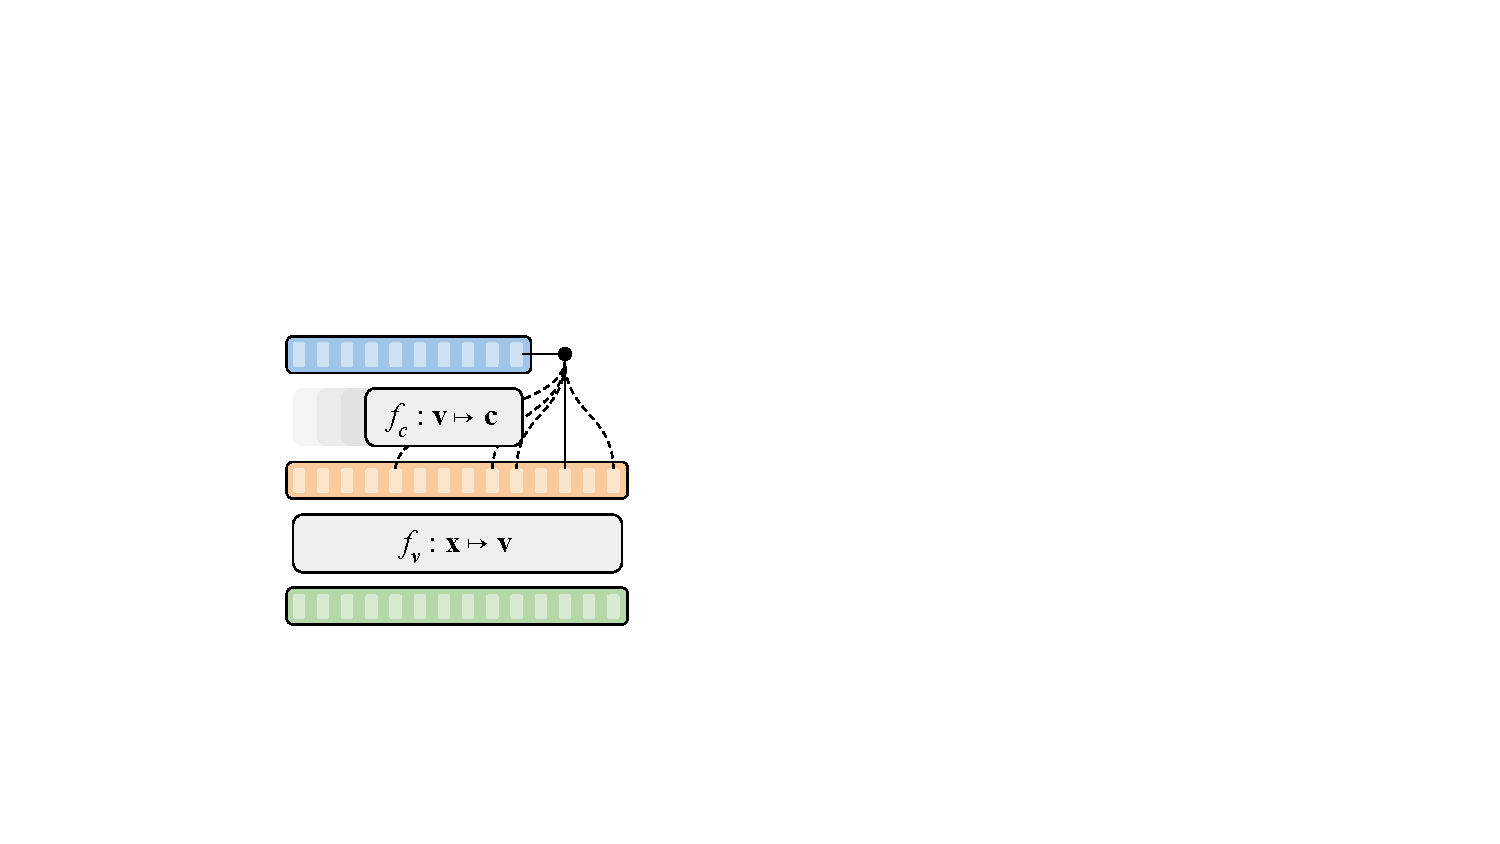
\includegraphics[width=0.40\textwidth]{../graphics/paper_brief/CON_PRD.pdf} & 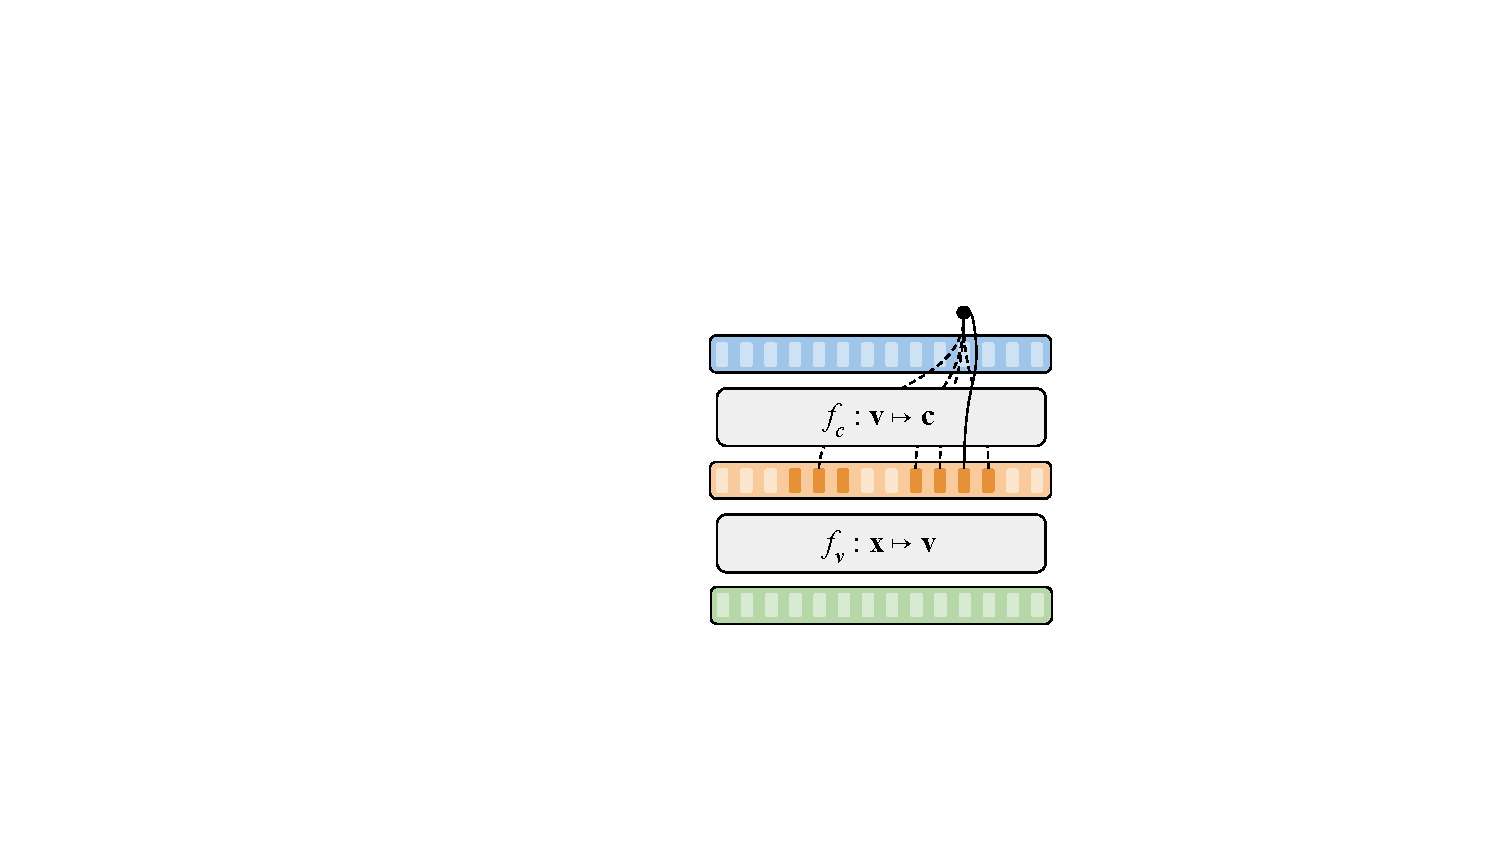
\includegraphics[width=0.40\textwidth]{../graphics/paper_brief/CON_MSK.pdf}
        \end{tabular}
        }
    \end{figure}
\end{frame}


\begin{frame}
    \frametitle{Overview: Representation Learning for Speech}

    \begin{columns}

        \begin{column}{0.4\textwidth}
            \begin{itemize}
                \item We focus on two primary categories:
                \begin{itemize}
                    \item Self-supervised learning (SSL)
                    \item Probabilistic latent variable models (LVMs)
                \end{itemize}
                \item Recent developments have been driven by self-supervised learning.
                \item A model-by-model overview: Focus on speech recognition.
            \end{itemize}
        \end{column}

        \begin{column}{0.6\textwidth}

            \begin{tikzpicture}
                \only<1->{
                    \node[anchor=south west,inner sep=0] (A) at (0,0) {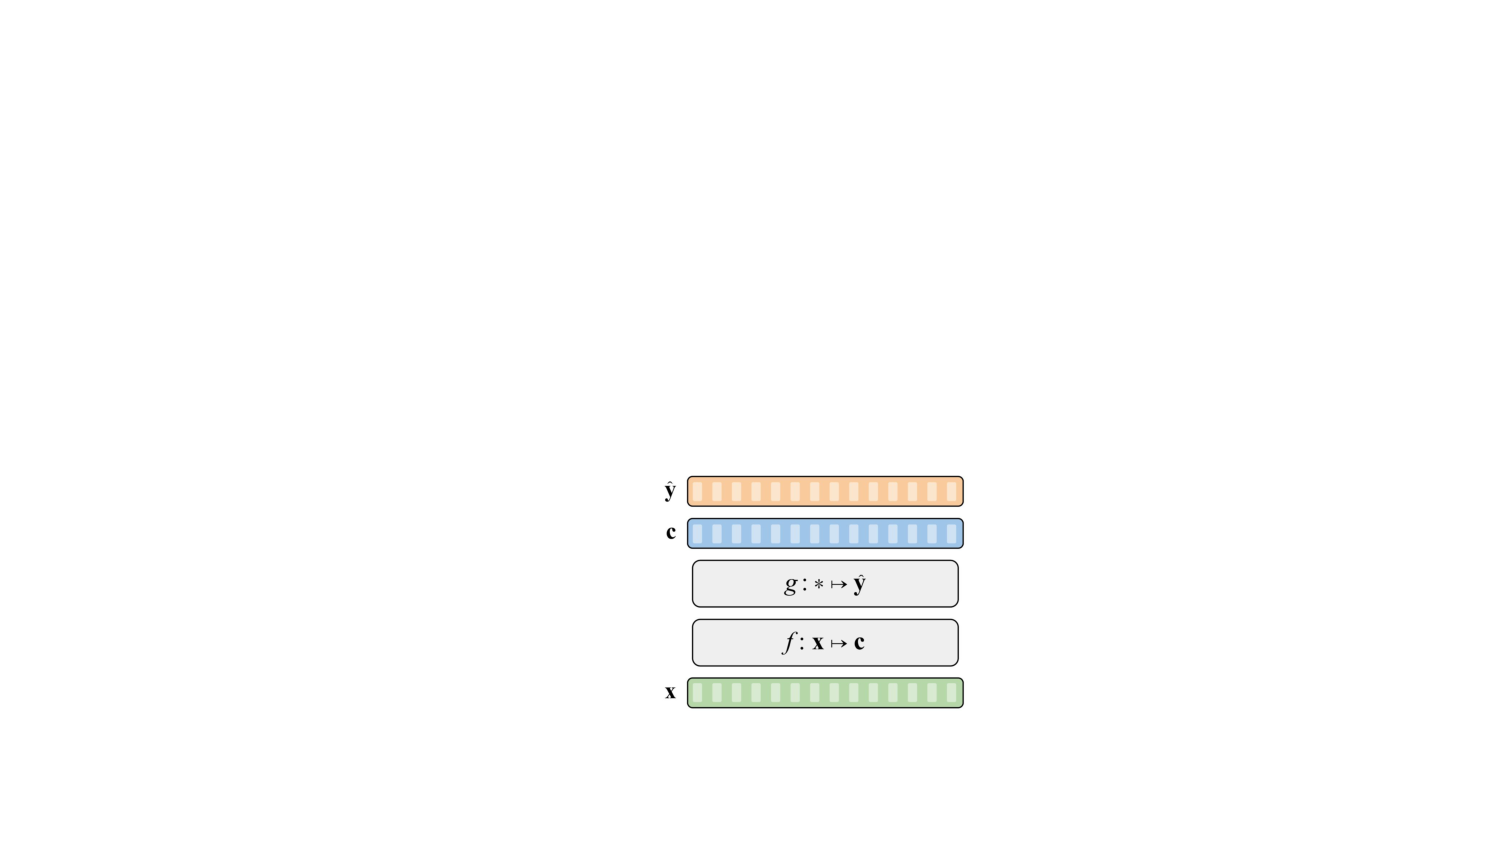
\includegraphics[height=0.4\textheight]{figures/brief-paradigms-ssl.pdf}};
                    \node[anchor=south west,inner sep=0] (B) at (4.2,0) {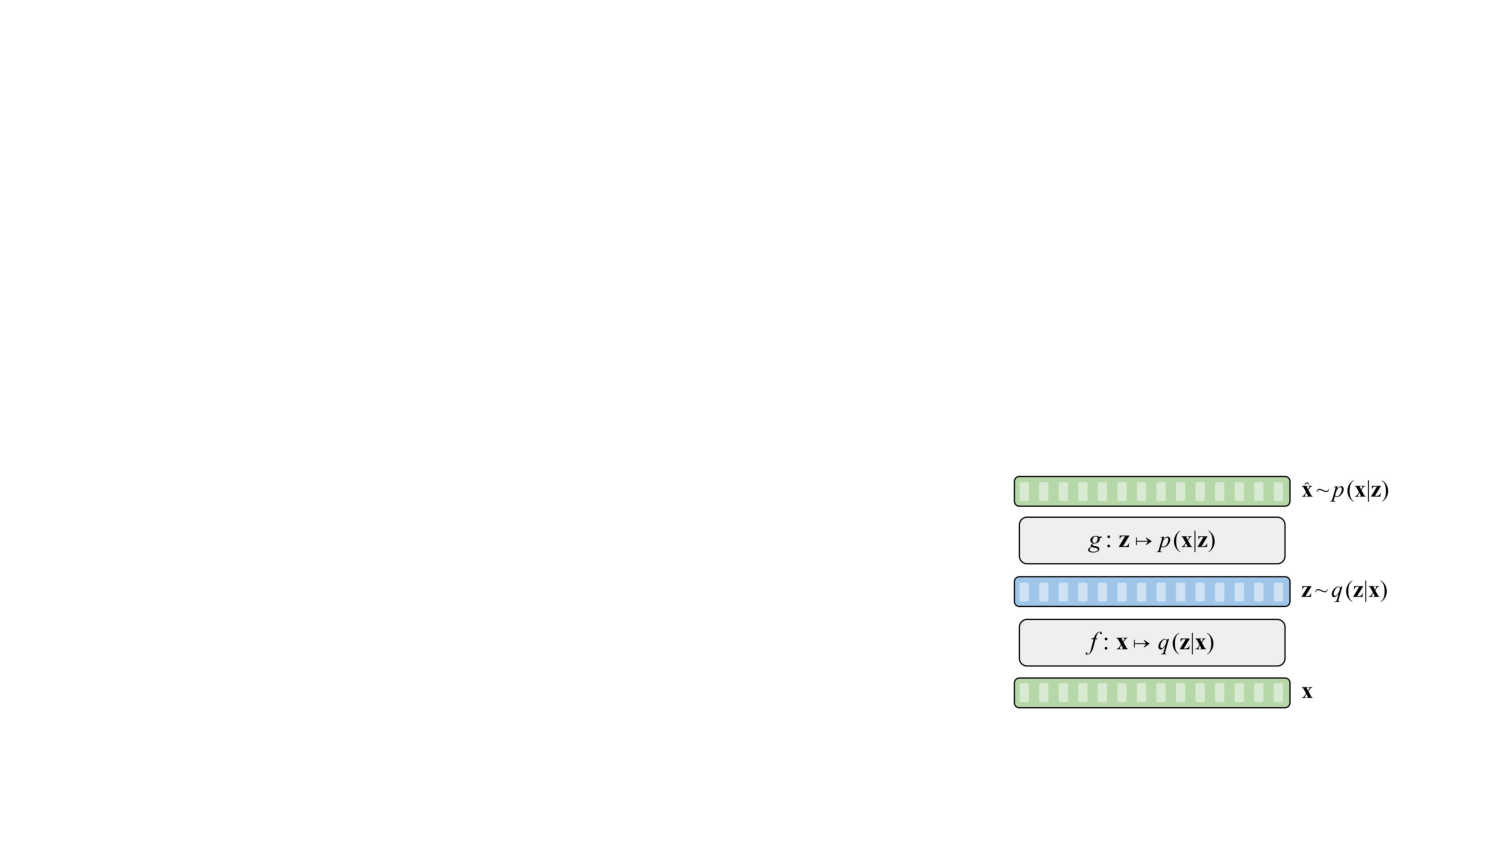
\includegraphics[height=0.4\textheight]{figures/brief-paradigms-lvm-2.pdf}};
                    \fill [draw=none, fill=white, fill opacity=0.7] (B.north west) -- (B.north east) -- (B.south east) -- (B.south west) -- (B.north west) -- cycle;
                }

                \only<2->{
                    \node[anchor=south west,inner sep=0] (A) at (0,0) {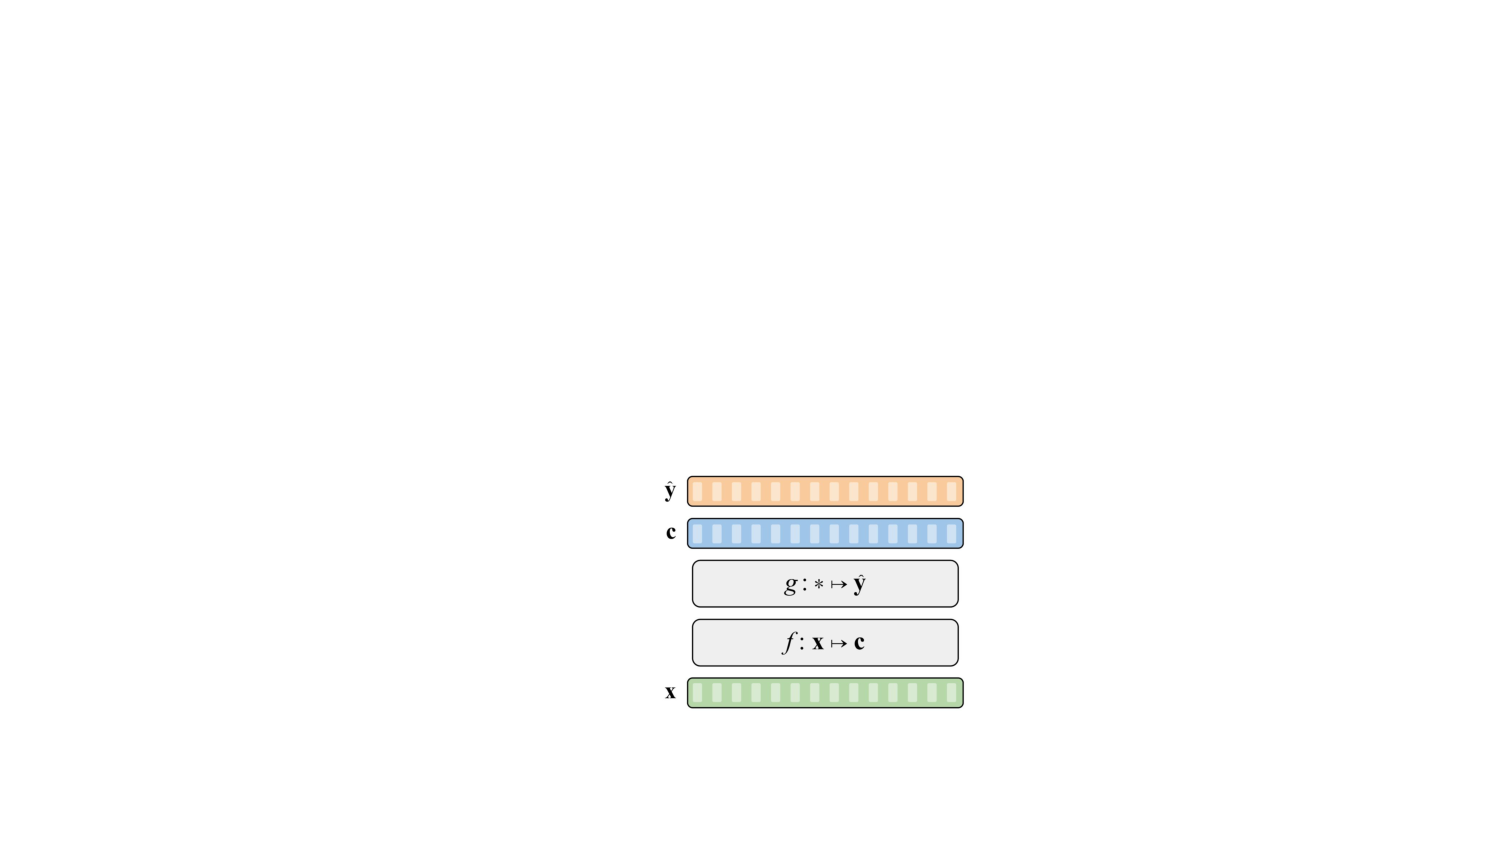
\includegraphics[height=0.4\textheight]{figures/brief-paradigms-ssl.pdf}};
                    \node[anchor=south west,inner sep=0] (B) at (4.2,0) {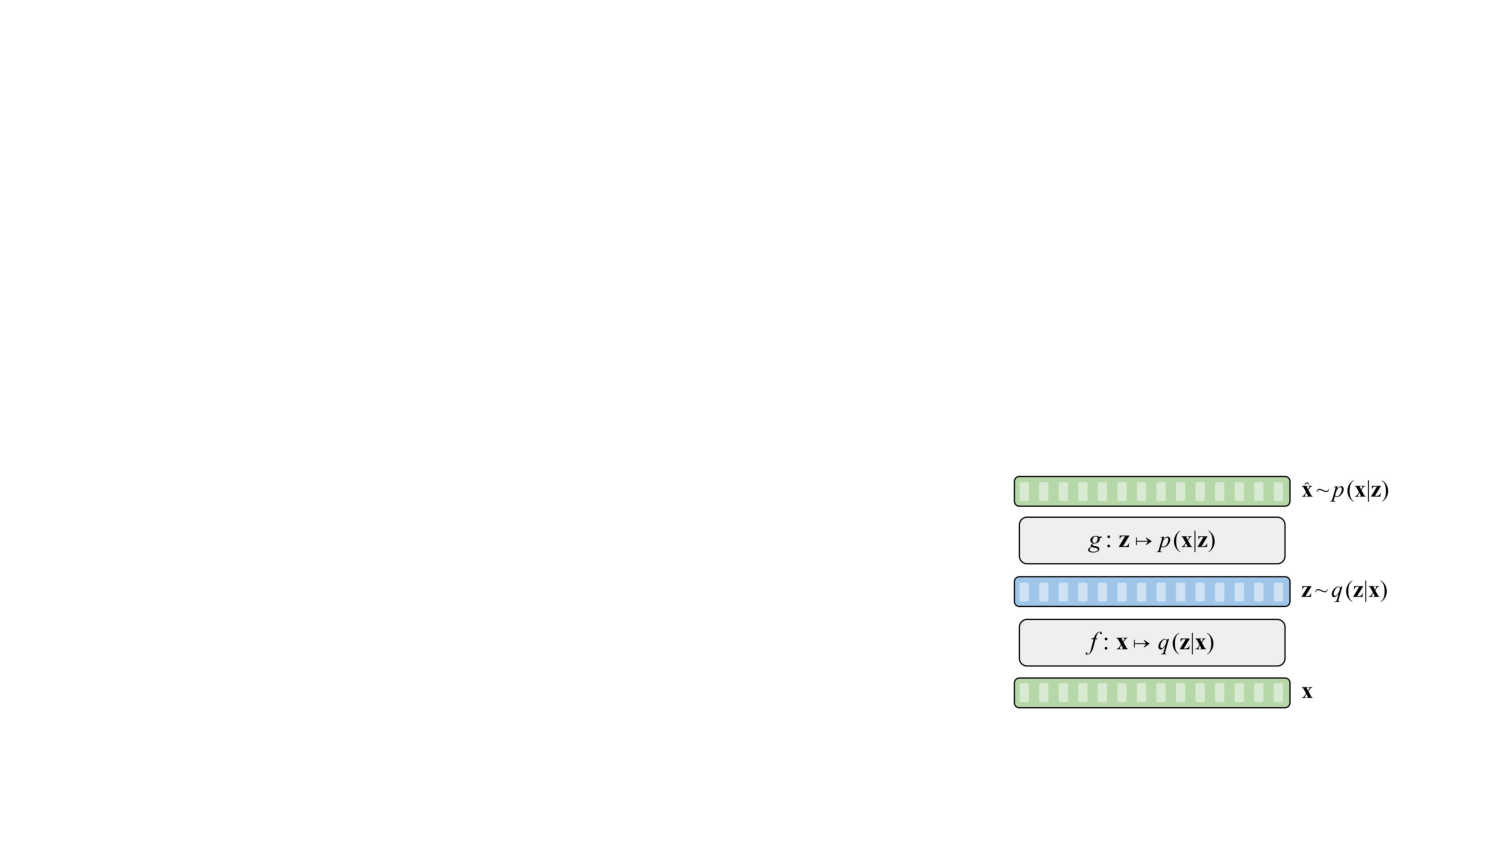
\includegraphics[height=0.4\textheight]{figures/brief-paradigms-lvm-2.pdf}};
                    \fill [draw=none, fill=white, fill opacity=0.7] (A.north west) -- (A.north east) -- (A.south east) -- (A.south west) -- (A.north west) -- cycle;
                }
            \end{tikzpicture}

        \end{column}
        
    \end{columns}
\end{frame}


\begin{frame}
    \frametitle{Graphical models for LVMs}
    % Figure TikZ sources at https://www.overleaf.com/project/61b212df9f315b5aec2b4a33
    \begin{columns}

        \begin{column}{0.5\textwidth}
            \begin{figure}
                \centering
                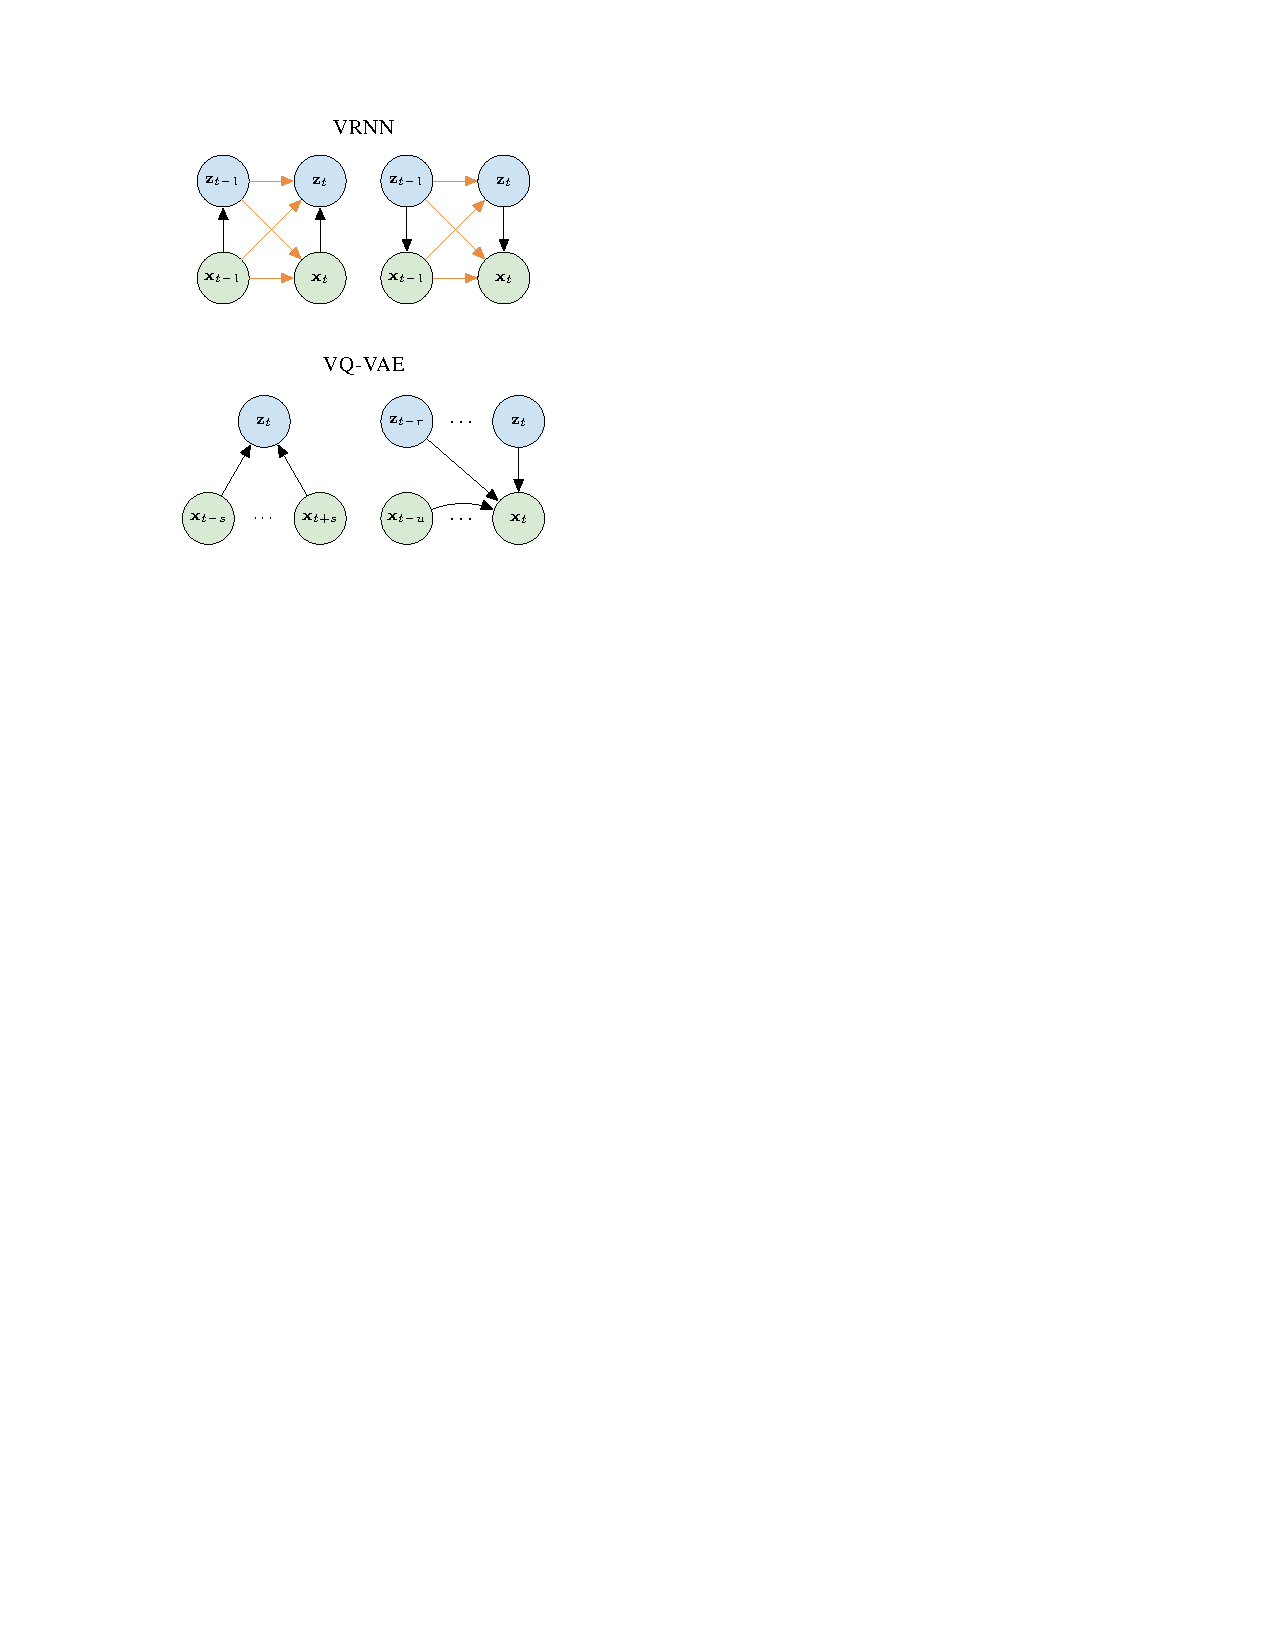
\includegraphics[width=0.8\textwidth]{figures/brief-vrnn-vqvae.pdf}
            \end{figure}
        \end{column}

        \begin{column}{0.5\textwidth}
            \begin{figure}
                \centering
                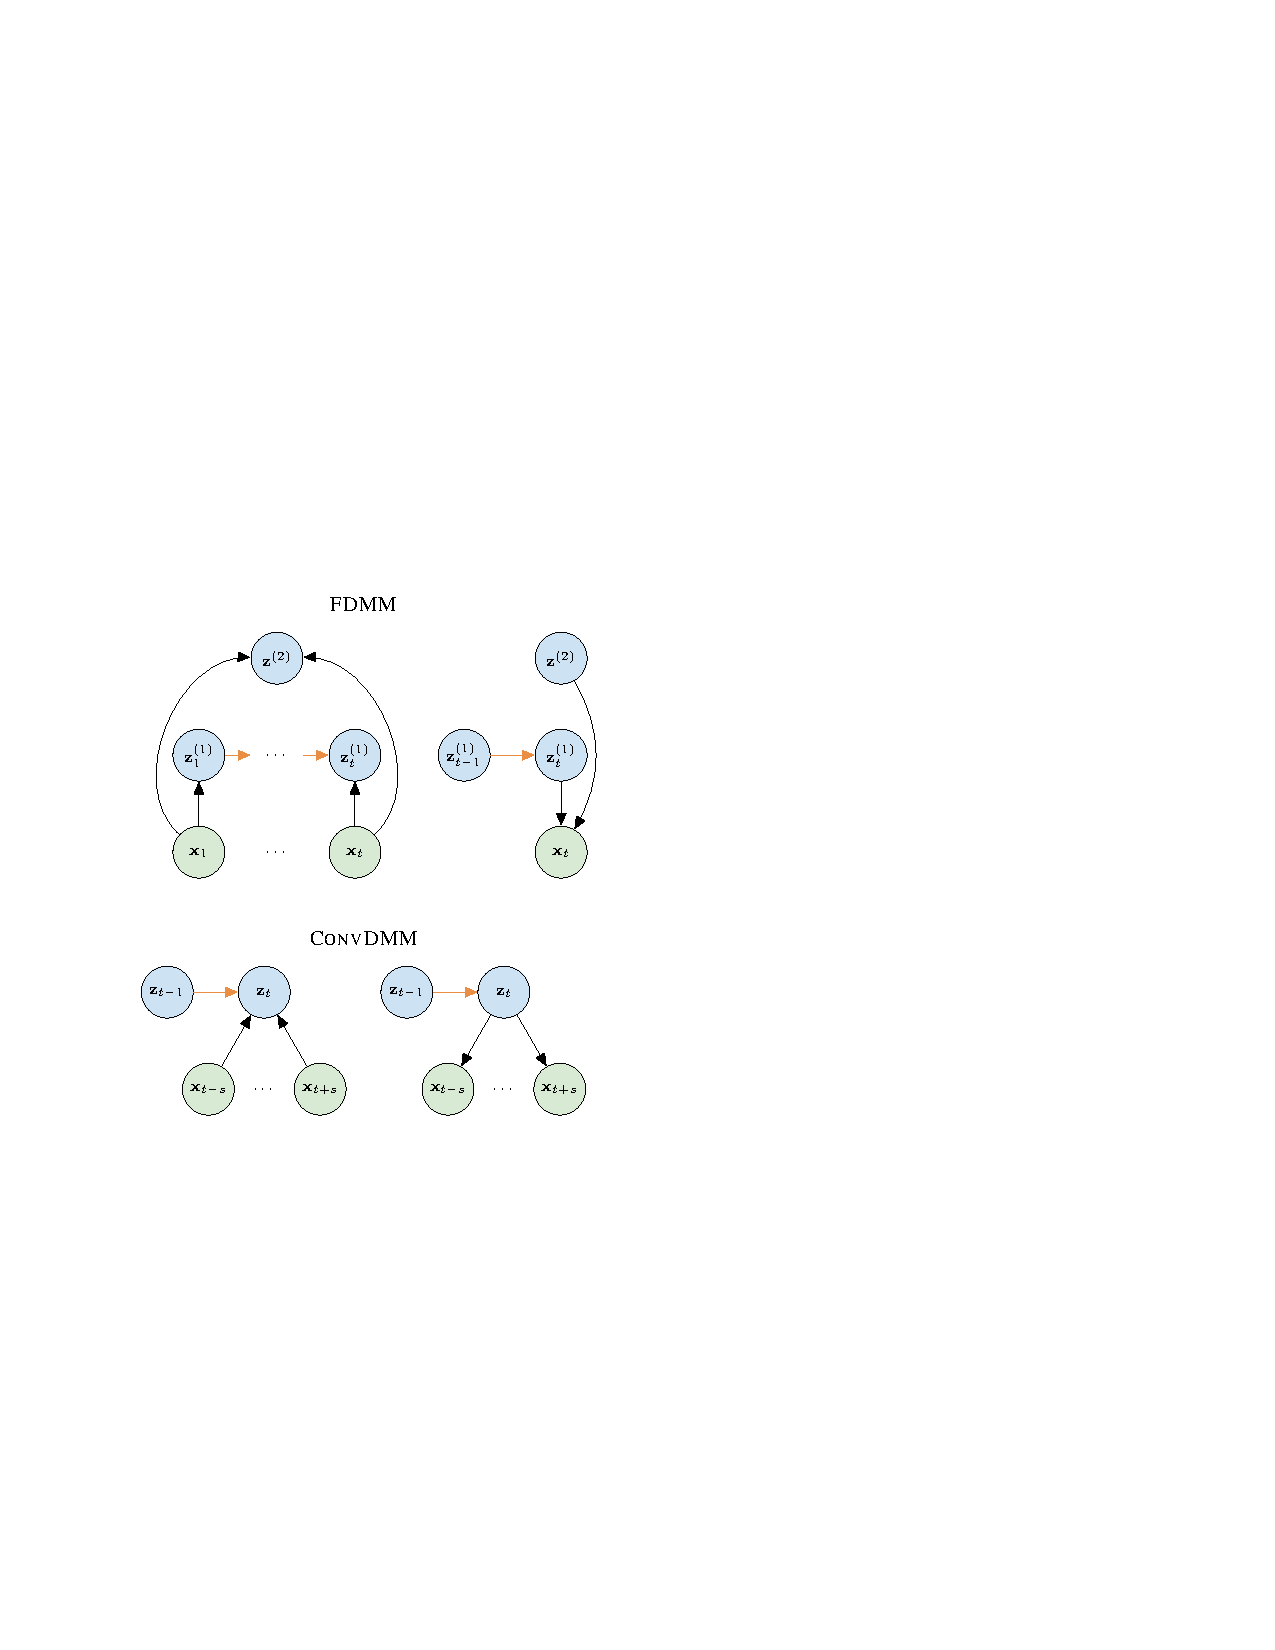
\includegraphics[width=0.8\textwidth]{figures/brief-fdmm-convdmm.pdf}
            \end{figure}            
        \end{column}

    \end{columns}

    \definecolor{sharedcolor}{RGB}{234 142 67} % mørk orange
    \blfootnote{\scalebox{0.6}{{\color{sharedcolor} Orange edges} indicate parameters shared between inference and generative models.}}
\end{frame}


\begin{frame}
    \frametitle{Overview of LVM probabilistic components}

    \begin{table}
        \centering
        \resizebox{0.8\textheight}{!}{%
            \begin{tabular}{ l l l } 
                \toprule
                \multicolumn{2}{l}{\textbf{\textsc{Type}}} & \textbf{\textsc{Form}} \\
                \midrule
                \multicolumn{3}{c}{\textsc{Observation model}} \\
                \midrule
                \textbf{\textsc{arx}} & Autoregressive on $\mathbf{x}_t$      & $p(\mathbf{x}_t|\mathbf{x}_{1:t-1})$ \\
                \textbf{\textsc{loc}} & Local latent variable                 & $p(\mathbf{x}_{t}|\mathbf{z}_{1:t})$ \\
                \textbf{\textsc{glb}} & Global latent variable                & $p(\mathbf{x}_{t}|\mathbf{z})$ \\
                \midrule
                \multicolumn{3}{c}{\textsc{Prior}} \\
                \midrule
                \textbf{\textsc{arx}} & Autoregressive on $\mathbf{x}_t$      & $p(\mathbf{z}_t|\mathbf{x}_{1:t-1})$ \\
                \textbf{\textsc{arz}} & Autoregressive on $\mathbf{z}_t$      & $p(\mathbf{z}_t|\mathbf{z}_{1:t-1})$ \\
                \textbf{\textsc{ind}} & Locally independent $\mathbf{z}_t$                 & $p(\mathbf{z}_t)$ \\
                \textbf{\textsc{glb}} & Global latent variable                & $p(\mathbf{z})$ \\
                \midrule
                \multicolumn{3}{c}{\textsc{Inference model}} \\
                \midrule
                \textbf{\textsc{arz}} & Autoregressive on $\mathbf{z}_t$      & $q(\mathbf{z}_t|\mathbf{z}_{1:t-1})$ \\
                \textbf{\textsc{flt}} & Filtering                             & $q(\mathbf{z}_t|\mathbf{x}_{1:t})$ \\
                \textbf{\textsc{lsm}} & Local smoothing                       & $q(\mathbf{z}_t|\mathbf{x}_{t-r:t+r})$ \\
                \textbf{\textsc{gsm}} & Global smoothing                      & $q(\mathbf{z}_t|\mathbf{x}_{1:T})$ \\
                \textbf{\textsc{glb}} & Global latent variable                & $q(\mathbf{z}|\mathbf{x}_{1:T})$ \\
                \bottomrule
            \end{tabular}
        }
    \end{table}

\end{frame}


\begin{frame}
    \frametitle{Classification of selected LVMs for speech}

    \begin{table}
        \centering
        \setlength{\tabcolsep}{3pt}
        \renewcommand{\arraystretch}{1.1}
        \resizebox{0.7\textwidth}{!}{%
            \begin{tabular}{ l | c c c | c c c c | c c c c c | c } 
                \toprule
                \multicolumn{2}{c}{} & 
                \multicolumn{3}{c}{\textsc{Observation}} & 
                \multicolumn{4}{c}{\textsc{Prior}} & 
                \multicolumn{5}{c}{\textsc{Inference}} \\
                \textbf{\textsc{model}} & 
                \textbf{\textsc{arx}} & 
                \textbf{\textsc{loc}} & 
                \textbf{\textsc{glb}} &  
                \textbf{\textsc{arx}} & 
                \textbf{\textsc{arz}} & 
                \textbf{\textsc{ind}} & 
                \textbf{\textsc{glb}} &  
                \textbf{\textsc{arz}} & 
                \textbf{\textsc{flt}} & 
                \textbf{\textsc{lsm}} & 
                \textbf{\textsc{gsm}} & 
                \textbf{\textsc{glb}} &
                \textbf{\textsc{hie}} \\
                \midrule
                %                                                              OBSERVATION       |              PRIOR                |                  INFERENCE       
                %                                                         ARX      LOC      GLB      ARX      ARZ     IND      GLB      ARZ      FLT      LSM      GSM      GLB
                \textbf{VRNN} \footnotesize{\parencite{chung_recurrent_2015}}          & \cmark & \cmark & \xmark & \cmark & \cmark & \xmark & \xmark & \cmark & \cmark & \xmark & \xmark & \xmark & \xmark \\
                \textbf{SRNN} \footnotesize{\parencite{fraccaro_sequential_2016}}      & \cmark & \cmark & \xmark & \cmark & \cmark & \xmark & \xmark & \cmark & \xmark & \xmark & \cmark & \xmark & \xmark \\
                \textbf{HMM-VAE} \footnotesize{\parencite{ebbers_hidden_2017}}         & \xmark & \cmark & \xmark & \xmark & \cmark & \xmark & \xmark & \cmark & \cmark & \xmark & \xmark & \xmark & \cmark \\
                \textbf{ConvVAE} \footnotesize{\parencite{hsu_learning_2017}}          & \xmark & \xmark & \cmark & \xmark & \xmark & \xmark & \cmark & \xmark & \xmark & \xmark & \cmark & \cmark & \xmark \\
                \textbf{FHVAE} \footnotesize{\parencite{hsu_unsupervised_2017}}        & \xmark & \cmark & \cmark & \xmark & \xmark & \cmark & \cmark & \xmark & \xmark & \xmark & \cmark & \cmark & \cmark \\
                \textbf{VQ-VAE} \footnotesize{\parencite{oord_neural_2018}}            & \cmark & \cmark & \xmark & \xmark & \xmark & \cmark & \xmark & \xmark & \xmark & \cmark & \xmark & \xmark & \xmark \\
                \textbf{BHMM-VAE} \footnotesize{\parencite{glarner_full_2018}}         & \xmark & \cmark & \xmark & \xmark & \cmark & \xmark & \xmark & \cmark & \cmark & \xmark & \xmark & \xmark & \xmark \\
                \textbf{STCN} \footnotesize{\parencite{aksan_stcn_2019}}               & \xmark & \cmark & \xmark & \cmark & \xmark & \xmark & \xmark & \xmark & \cmark & \xmark & \xmark & \xmark & \cmark \\
                \textbf{FDMM} \footnotesize{\parencite{khurana_factorial_2019}}        & \xmark & \cmark & \cmark & \xmark & \cmark & \xmark & \cmark & \cmark & \cmark & \xmark & \xmark & \cmark & \cmark \\
                \textbf{ConvDMM} \footnotesize{\parencite{khurana_convolutional_2020}} & \xmark & \cmark & \xmark & \xmark & \cmark & \xmark & \xmark & \cmark & \xmark & \cmark & \xmark & \xmark & \xmark \\
                \bottomrule
            \end{tabular}
        }
    \end{table}

\end{frame}

\begin{frame}
    \frametitle{Comparison of LVMs and SSL methods}

    \begin{table}
        \centering
        \setlength{\tabcolsep}{3pt}
        \renewcommand{\arraystretch}{1.1}
        \resizebox{1\textheight}{!}{%
            \begin{tabular}{ l l | c c c c c c | c c c | c c } 
                \toprule
                
                \multicolumn{2}{c}{} & 
                \multicolumn{6}{c}{\textsc{model and task design}} & 
                \multicolumn{3}{c}{\textsc{resolution}} &
                \multicolumn{2}{c}{\makebox[0pt][c]{\textsc{usage}}} \\
                & \textbf{\textsc{model}} &
                \textbf{\textsc{msk}} & 
                \textbf{\textsc{prd}} & 
                \textbf{\textsc{con}} &  
                \textbf{\textsc{rec}} &  
                \textbf{\textsc{qtz}} & 
                \textbf{\textsc{gen}} & 
                \textbf{\textsc{loc}} & 
                \textbf{\textsc{glb}} & 
                \textbf{\textsc{var}} & 
                \textbf{\textsc{frz}} & 
                \textbf{\textsc{ftn}} \\
                
                \midrule
                % \multicolumn{11}{c}{\textsc{Self-supervised models}} \\
                % \midrule
                %                                                           MSK      PRD      CON      REC      QTZ      GEN      LOC      GLB     VAR      FRZ      FTN
                \verticalmultirow{9}{\textsc{Self-supervised models}} 
                % & \textbf{Audio Word2vec} \footnotesize{\parencite{chung_audio_2016}}      & \cmark & \xmark & \xmark & \cmark & \xmark & \xmark & \xmark & \cmark & \xmark & \cmark & \xmark \\
                % & \textbf{Speech2Vec} \footnotesize{\parencite{chung_speech2vec_2018}}     & \xmark & \cmark & \xmark & \cmark & \xmark & \xmark & \xmark & \cmark & \xmark & \cmark & \xmark \\
                % & \textbf{Unspeech} \footnotesize{\parencite{milde_unspeech_2018}}         & \xmark & \cmark & \cmark & \xmark & \xmark & \xmark & \xmark & \cmark & \xmark & \cmark & \xmark \\
                
                & \textbf{CPC} \footnotesize{\parencite{oord_representation_2018}}         & \xmark & \cmark & \cmark & \xmark & \xmark & \xmark & \cmark & \xmark & \xmark & \cmark & \xmark \\
                
                & \textbf{APC} \footnotesize{\parencite{chung_unsupervised_2019}}          & \xmark & \cmark & \xmark & \cmark & \xmark & \xmark & \cmark & \xmark & \xmark & \cmark & \xmark \\ % 5/4
                & \textbf{wav2vec} \footnotesize{\parencite{schneider_wav2vec_2019}}       & \xmark & \cmark & \cmark & \xmark & \xmark & \xmark & \cmark & \xmark & \xmark & \cmark & \xmark \\ % 11/4
                & \textbf{Mockingjay}  \footnotesize{\parencite{liu_mockingjay_2020}}      & \cmark & \xmark & \xmark & \cmark & \xmark & \xmark & \cmark & \xmark & \xmark & \cmark & \cmark \\ % 25/10-19
                & \textbf{wav2vec 2.0} \footnotesize{\parencite{baevski_wav2vec_2020}}     & \cmark & \xmark & \cmark & \xmark & \cmark & \xmark & \cmark & \xmark & \xmark & \xmark & \cmark \\ % 20/6
                & \textbf{NPC} \footnotesize{\parencite{liu_nonautoregressive_2020}}       & \cmark & \xmark & \xmark & \cmark & \cmark & \xmark & \cmark & \xmark & \xmark & \cmark & \xmark \\ % 1/11
                & \textbf{DeCoAR 2.0} \footnotesize{\parencite{ling_decoar_2020}}          & \cmark & \xmark & \xmark & \cmark & \cmark & \xmark & \cmark & \xmark & \xmark & \cmark & \xmark \\ % 11/12
                % & \textbf{SCPC} \footnotesize{\parencite{bhati_segmental_2021}}            & \xmark & \cmark & \cmark & \xmark & \xmark & \xmark & \cmark & \xmark & \cmark & \cmark & \xmark \\ % 3/6
                & \textbf{HuBERT} \footnotesize{\parencite{hsu_hubert_2021}}               & \cmark & \xmark & \xmark & \xmark & \cmark & \xmark & \cmark & \xmark & \xmark & \xmark & \cmark \\ % 14/6
                & \textbf{data2vec} \footnotesize{\parencite{baevski_data2vec_2022}}       & \cmark & \xmark & \xmark & \xmark & \xmark & \xmark & \cmark & \xmark & \xmark & \xmark & \cmark \\ % 16/6

                \midrule
                % \multicolumn{11}{c}{\textsc{Probabilistic latent variable models}} \\
                % \midrule
                %                                                           MSK      PRD      CON      REC      QTZ      GEN      LOC      GLO     VAR      FRZ      FTN
                \verticalmultirow{8}{\textsc{Latent variable models}}
                & \textbf{VRNN} \footnotesize{\parencite{chung_recurrent_2015}}          & \xmark & \xmark & \xmark & \cmark & \xmark & \cmark & \cmark & \xmark & \xmark & \cmark & \xmark \\
                & \textbf{SRNN} \footnotesize{\parencite{fraccaro_sequential_2016}}      &\xmark & \xmark & \xmark & \cmark & \xmark & \cmark & \cmark & \xmark & \xmark & \cmark & \xmark \\
                % & \textbf{HMM-VAE} \footnotesize{\parencite{ebbers_hidden_2017}}         & \xmark & \xmark & \xmark & \cmark & \xmark & \cmark & \cmark & \xmark & \xmark & \cmark & \xmark \\
                & \textbf{ConvVAE} \footnotesize{\parencite{hsu_learning_2017}}          & \xmark & \xmark & \xmark & \cmark & \xmark & \cmark & \xmark & \cmark & \xmark & \cmark & \xmark \\
                & \textbf{FHVAE} \footnotesize{\parencite{hsu_unsupervised_2017}}        & \xmark & \xmark & \xmark & \cmark & \xmark & \cmark & \cmark & \cmark & \xmark & \cmark & \xmark \\
                & \textbf{VQ-VAE} \footnotesize{\parencite{oord_neural_2018}}            & \xmark & \xmark & \xmark & \cmark & \cmark & \cmark & \cmark & \xmark & \xmark & \cmark & \xmark \\
                % & \textbf{BHMM-VAE} \footnotesize{\parencite{glarner_full_2018}}         & \xmark & \xmark & \xmark & \cmark & \xmark & \cmark & \cmark & \xmark & \xmark & \cmark & \xmark \\
                & \textbf{STCN} \footnotesize{\parencite{aksan_stcn_2019}}               & \xmark & \xmark & \xmark & \cmark & \xmark & \cmark & \cmark & \xmark & \xmark & \cmark & \xmark \\
                & \textbf{FDMM} \footnotesize{\parencite{khurana_factorial_2019}}        & \xmark & \xmark & \xmark & \cmark & \xmark & \cmark & \cmark & \cmark & \xmark & \cmark & \xmark \\
                & \textbf{ConvDMM} \footnotesize{\parencite{khurana_convolutional_2020}} & \xmark & \xmark & \xmark & \cmark & \xmark & \cmark & \cmark & \xmark & \xmark & \cmark & \xmark \\
                \bottomrule
            \end{tabular}
        }
    \end{table}

\end{frame}


% ======================================================================================================================


\subsection[A Retrospective Study on Machine Learning-Assisted Stroke Recognition for Medical Helpline Calls]{a retrospective study on machine learning-assisted stroke recognition for medical helpline calls}


\begin{frame}
    \frametitle{Simulated prospective study}
    \begin{enumerate}
        \item[I.] \highlight{When} is the model prediction presented to the call-taker?
        \begin{enumerate}
            \item[1.] Notify the call-taker \highlight{after the call ends}.
            \item[2.] Notify the call-taker \highlight{during the call}.
        \end{enumerate}
        \item[II.] \highlight{How} does prediction influence the diagnostic code the call-taker assigns to the call?
        \begin{enumerate}[label=\Alph*.]
            \item[A.] Call-takers \highlight{mirror model positives}.
            \item[B.] Call-takers \highlight{mirror model negatives}.
            \item[C.] Call-takers mirror model predictions (corresponds to main results of the model itself).
        \end{enumerate}
    \end{enumerate}
    \vspace{0.5em}
    To simulate the online scenario (2.), we \highlight{stream the transcript} to the model and make predictions every 50 words. 
    A stroke positive is triggered only when three consecutive positive predictions are made. 
    This is similar to the strategy implemented for a previous RCT on cardiac arrest \cite{cite15}.

        % %
        % Option 1 is identical to the method used in the main study. In option 2, predictions are made during the call based only on partial transcriptions. We implemented option 2 in such a manner that the model predicted every time 50 new words were transcribed and added to the transcript. A stroke positive was triggered only when three consecutive positive predictions were made (i.e., without intermediate negative stroke predictions). In other words, the sigmoid activation of the model had to remain above 0.5 for three consecutive predictions, for example, after 150, 200, and 250 words were transcribed.
        
        % As we can only assume how call takers are influenced by model predictions (II), precisely evaluating the hypothetical performance of call takers when supported by a machine learning framework is impossible. Furthermore, option 2 may influence the conversation, further complicating matters. Therefore, we report the results combining the call taker and the model under the following two assumptions:
        % %
\end{frame}


\begin{frame}
    \frametitle{Simulated prospective study}

    \begin{table}
        \centering
        \resizebox*{0.98\textwidth}{!}{%
        \begin{tabular}{l|c|cc|cc|cc}
            \toprule
    
            \textbf{Predictor} & \textbf{Call-taker} & \multicolumn{2}{c|}{\textbf{Model}} & \multicolumn{4}{c}{\textbf{Call-taker supported by the model (simulated)}} \\
            \midrule
            \textbf{When} & \textbf{During call} & \textbf{After call} & \textbf{During call} & \textbf{After call} & \textbf{During call} & \textbf{After call} & \textbf{During call} \\
            \midrule
            \textbf{Method} & - & - & - & \textbf{neg $\rightarrow$ pos} & \textbf{neg $\rightarrow$ pos} & \textbf{pos $\rightarrow$ neg} & \textbf{pos $\rightarrow$ neg} \\
            \midrule
    
            \makecell[l]{\textbf{F1-score} [\%] $\uparrow$}                             & \makecell[c]{25.8 \\ \shade{(23.7-27.9)}} & \makecell[c]{35.7 \\ \shade{(35.0-36.4)}} & \makecell[c]{33.1 \\ \shade{(32.4-33.7)}} & \makecell[c]{28.9 \\ \shade{(28.3-29.5)}} & \makecell[c]{27.6 \\ \shade{(27.0-28.1)}}  & \makecell[c]{33.3 \\ \shade{(32.5-34.1)}}& \makecell[c]{32.7 \\ \shade{(31.8-33.5)}} \\
            \midrule
            \makecell[l]{\textbf{Sensitivity} [\%] $\uparrow$}                          & \makecell[c]{52.7 \\ \shade{(49.2-56.4)}} & \makecell[c]{63.0 \\ \shade{(62.0-64.1)}} & \makecell[c]{58.7 \\ \shade{(57.7-59.8)}} & \makecell[c]{72.4 \\ \shade{(71.5-73.3)}} & \makecell[c]{72.3 \\ \shade{(71.4-73.3)}} & \makecell[c]{43.4 \\ \shade{(42.3-44.5)}} & \makecell[c]{39.1 \\ \shade{(38.1-40.1)}} \\
            \midrule
            \makecell[l]{\textbf{PPV} [\%] $\uparrow$}                                  & \makecell[c]{17.1 \\ \shade{(15.5-18.6)}} & \makecell[c]{24.9 \\ \shade{(24.3-25.5)}} & \makecell[c]{23.0 \\ \shade{(22.5-23.6)}} & \makecell[c]{18.0 \\ \shade{(17.6-18.4)}} & \makecell[c]{17.0 \\ \shade{(16.7-17.4)}} & \makecell[c]{27.0 \\ \shade{(26.3-27.8)}} & \makecell[c]{28.1 \\ \shade{(27.3-28.9)}} \\
            \midrule
            \makecell[l]{\textbf{FOR} [\%] $\downarrow$\\ \shade{(1 - NPV)} }           & \makecell[c]{0.105 \\ \shade{(0.094-0.116)}} & \makecell[c]{0.082 \\ \shade{(0.079-0.085)}} & \makecell[c]{0.091 \\ \shade{(0.088-0.094)}} & \makecell[c]{0.061 \\ \shade{(0.059-0.064)}} & \makecell[c]{0.061 \\ \shade{(0.059-0.064)}} & \makecell[c]{0.125 \\ \shade{(0.121-0.129)}} & \makecell[c]{0.134 \\ \shade{(0.131-0.138)}} \\
            \midrule
            \makecell[l]{\textbf{FPR} [\%] $\downarrow$\\ \shade{(1 - specificity)} }   & \makecell[c]{0.565 \\ \shade{(0.539-0.590)}} & \makecell[c]{0.419 \\ \shade{(0.413-0.426)}} & \makecell[c]{0.432 \\ \shade{(0.426-0.439)}} & \makecell[c]{0.726 \\ \shade{(0.717-0.735)}} & \makecell[c]{0.776 \\ \shade{(0.767-0.786)}} & \makecell[c]{0.258 \\ \shade{(0.253-0.263)}} & \makecell[c]{0.221 \\ \shade{(0.216-0.226)}} \\
    
            \bottomrule
        \end{tabular}%
        }
    \end{table}
\end{frame}


\begin{frame}
    \frametitle{Fine-tuning a large language model}
    \begin{itemize}
        \item Large language models are effective in a wide range of NLP tasks \cite{devlin_bert_2018, radford_improving_2018}.
        \item Might BERT be useful for recognizing stroke?
    \end{itemize}
    \begin{table}
        \centering
        \resizebox*{0.95\textwidth}{!}{%
        \begin{tabular}{ll|ccccc}
            \toprule
            \textbf{Subset} & \textbf{Predictor} & \textbf{F1-score [\%] $\uparrow$} & \textbf{Sensitivity [\%] $\uparrow$} & \textbf{PPV [\%] $\uparrow$} & \makecell[c]{\textbf{FOR [\%] $\downarrow$} \\ (1 - NPV)} & \makecell[c]{\textbf{FPR [\%] $\downarrow$} \\ (1 - specificity)} \\
            \midrule
            \verticalmultirow{3}{\emph{Overall}} & \textbf{Call-takers}                        & \makecell[c]{25.8 \shade{(23.7-27.9)}} & \makecell[c]{52.7 \shade{(49.2-56.4)}} & \makecell[c]{17.1 \shade{(15.5-18.6)}} & \makecell[c]{0.105 \shade{(0.094-0.116)}} & \makecell[c]{0.565 \shade{(0.539-0.590)}} \\
                                                    & \makecell[l]{\textbf{MLP}}                  & \makecell[c]{35.7 \shade{(35.0-36.4)}} & \makecell[c]{63.0 \shade{(62.0-64.1)}} & \makecell[c]{24.9 \shade{(24.3-25.5)}} & \makecell[c]{0.082 \shade{(0.079-0.085)}} & \makecell[c]{0.419 \shade{(0.413-0.426)}} \\
                                                    & \makecell[l]{\textbf{BERT} (fine-tuned)} & \makecell[c]{33.8 \shade{(31.5-36.2)}} & \makecell[c]{57.5 \shade{(53.9-60.9)}} & \makecell[c]{23.9 \shade{(21.9-25.9)}} & \makecell[c]{0.094 \shade{(0.084-0.104)}} & \makecell[c]{0.403 \shade{(0.381-0.424)}} \\
            \bottomrule
        \end{tabular}%
        }
    \end{table}
\end{frame}


% ======================================================================================================================


\subsection*{Overview}

\begin{frame}[allowframebreaks]
    \frametitle{Table of contents}
    \tableofcontents
\end{frame}
